% !TEX root = ../main.tex
\chapter{Open Quantum Systems} % Main chapter title
\label{chapter_open_quantum_systems} % Label for referencing this chapter

%------------------------------------------------------------------------------
%	SECTION 1: Introduction to Open Quantum Systems
%------------------------------------------------------------------------------

\section{Introduction to Open Quantum Systems}
\label{sec:introduction_open_quantum_systems}

Any real-world quantum system is not perfectly isolated. Instead, it interacts with its surrounding environment. Unlike theoretical closed quantum systems that evolve unitarily according to the Schrödinger equation, open quantum systems experience non-unitary evolution due to their coupling with an external environment or reservoir.
Whenever the system is driven out of equilibrium by external perturbations, this coupling makes the system relax back to equilibrium.
\subsection{What are Open Quantum Systems?}
Open quantum systems are quantum systems that interact with an external environment, often called a "bath," which typically has infinite degrees of freedom and is usually assumed to be in thermal equilibrium~\cite{breuerpetruccione2009theoryopenquantum, weiss2012quantumdissipativesystems}. This interaction leads to several fundamental phenomena that distinguish open systems from isolated, closed quantum systems.

A central effect is \textbf{decoherence}, where quantum superposition states lose their phase relationships due to entanglement with the environment (\textbf{dephasing}). As a result, pure quantum states evolve into classical statistical mixtures, and the system's ability to exhibit quantum interference is diminished. The characteristic time scale for this process, known as the \emph{coherence time}, is of utmost importance in experiments, especially in high-resolution spectroscopy, quantum information processing, and quantum optics. For example, in two-dimensional electronic spectroscopy, the coherence time determines the ability to resolve quantum beats and thus extract information about energy transfer pathways in complex molecular systems~\cite{mukamel1995principlesnonlinearoptical}.

In addition to dephasing, the system-environment interaction leads to \textbf{dissipation} or \textbf{thermalization}, where energy is exchanged between the system and its surroundings, causing the system to relax toward a thermal state determined by the environment's temperature.

Understanding and controlling these effects is crucial for the design of quantum technologies, such as quantum computers and sensors, where environmental noise can rapidly destroy fragile quantum states~\cite{laddetal2010quantumcomputers}.  \todoref{find better reference}.%schlosshauer2007decoherencebook?, 

In summary, open quantum systems theory provides the framework to describe how quantum systems lose their "quantumness" and transition toward classical behavior due to unavoidable interactions with their environment.

\subsection{Origins and Physical Motivation}

Open quantum systems theory emerges naturally from the realization that perfect isolation of quantum systems is practically impossible; every quantum system in nature interacts with its environment to some degree. For instance, atoms are subject to electromagnetic field fluctuations (vacuum fluctuations)~\cite{breuerpetruccione2009theoryopenquantum}, quantum dots in solid-state environments couple to phonon baths~\cite{weiss2012quantumdissipativesystems}, and molecular systems interact with surrounding solvent molecules~\cite{mukamel1995principlesnonlinearoptical}. Quantum computers are particularly sensitive to environmental noise, which can rapidly destroy quantum coherence~\cite{laddetal2010quantumcomputers}, while biological quantum systems such as photosynthetic complexes operate in inherently noisy cellular environments.%~ \todoref{schlosshauer2007decoherencebook}. 
These diverse scenarios all require a theoretical framework that accounts for the coexistence of quantum effects and environmental influences.


\subsection{Theoretical Approaches}

A variety of theoretical frameworks have been developed to describe the dynamics of open quantum systems, each with its own range of validity and underlying assumptions. The most important distinction among these approaches is whether they assume \textbf{Markovian} or \textbf{non-Markovian} dynamics.

\subsubsection{Markovian vs. Non-Markovian Dynamics}
\label{subsec:markovian_nonmarkovian}

\noindent
\textbf{Markovian dynamics} assume that the environment has no memory: the future evolution of the system depends only on its present state, not on its past history. This is valid when the environmental correlation time is much shorter than the system's characteristic timescale. In contrast, \textbf{non-Markovian dynamics} account for memory effects, where the environment retains information about the system's past, leading to feedback and more complex evolution~\cite{breuerpetruccione2009theoryopenquantum, rivasetal2014quantumnonmarkovianitycharacterization}.

\subsubsection{Overview of Main Approaches}

\paragraph{Stochastic Approaches}

\noindent
Stochastic Schrödinger equations and quantum trajectories unravel master equations into individual pure state evolutions, clarifying measurement backaction and quantum jumps~\cite{vogtetal2013stochasticblochredfieldtheory, breuerpetruccione2009theoryopenquantum, carmichael1993opensystemsapproach}.

\paragraph{Non-Markovian Approaches}

\noindent
Time-convolutionless and Nakajima–Zwanzig master equations introduce memory kernels to describe non-Markovian effects~\cite{breuerpetruccione2009theoryopenquantum, rivasetal2014quantumnonmarkovianitycharacterization}. The hierarchical equations of motion (HEOM) provide a numerically exact framework for strong coupling and non-Markovian, condensed-phase environments like liquids or solids~\cite{tanimura2020numericallyexactapproach}. This is the most computationally expensive method. Path-integral methods based on the Feynman–Vernon influence functional offer a non-perturbative route to non-Markovian dynamics~\cite{weiss2012quantumdissipativesystems}.

\paragraph{Master Equation Approaches}

\noindent
The Lindblad master equation (Markovian) gives a general form for completely positive, trace-preserving dynamics under the Markov approximation and is widely used in quantum optics and quantum information~\cite{breuerpetruccione2009theoryopenquantum, lindblad1976generatorsquantumdynamical}. The Redfield equation (Markovian but not always CPTP) follows from a microscopic Born–Markov derivation, captures dissipation and dephasing, and does not guarantee complete positivity~\cite{redfield1965theoryrelaxationprocesses, rivasetal2014quantumnonmarkovianitycharacterization, lietal2018conceptsquantumnonmarkovianity}.
\todoidea{explain why we choose the Redfield equation for this thesis ->  it represents the best compromise between accuracy and computational efficiency for our systems of interest.}


\subsection{The Redfield Equation: A Central Tool}

\noindent
Among the various master equation approaches to open quantum systems, the Redfield equation occupies a particularly important position due to its microscopic foundation and broad applicability~\cite{redfield1965theoryrelaxationprocesses, breuerpetruccione2009theoryopenquantum}.
Unlike phenomenological approaches that introduce dissipation and dephasing \emph{ad hoc}, the Redfield formalism derives these effects directly from the microscopic Hamiltonian of the total system~\cite{breuerpetruccione2009theoryopenquantum, weiss2012quantumdissipativesystems} and
relates them to environmental correlation functions or spectral densities.
Originally developed by A.G. Redfield in 1957 and 1965 for nuclear magnetic resonance relaxation phenomena~\cite{redfield1965theoryrelaxationprocesses}, the Redfield equation describes the time evolution of the reduced density matrix of a quantum system weakly coupled to a thermal environment.

\noindent
However, it is important to note that the Redfield equation, while preserving trace and Hermiticity, does not guarantee complete positivity of the density matrix—a fundamental requirement for physical quantum states~\cite{rivasetal2010markovianmasterequations}. This limitation restricts its validity to the weak-coupling regime and requires careful analysis of its applicability in specific physical situations. In practice, the Redfield approach assumes weak system--environment coupling (Born, small $\alpha$) and a bath correlation time much shorter than system time scales (Markov).

\noindent
The following requirements must be fulfilled by the final derived Redfield equation:

\begin{enumerate}
	\item The equation should be linear in the system density matrix $\dot{\rho}_S(t) = F(\rho_S(t))$ (reduced equation of motion).
	\item The equation should be Markovian, meaning that the evolution of the system density matrix at time $t$ only depends on the state of the system at time $t$ and not on its past history.
	\item The equation should be trace-preserving, meaning that $\mathrm{Tr}[\rho_S(t)] = \mathrm{Tr}[\rho_S(0)]$ for all times $t$.
\end{enumerate}

\noindent
Unlike the Lindblad equation, the Redfield equation does not guarantee the complete positivity of the density matrix, which is a requirement for a physical state. Care must be taken when determining when the Redfield equation is useful. The equation will be valid in the weak coupling limit, meaning that the coupling strength in the interaction Hamiltonian fulfills $\alpha \ll 1$.



\noindent
In this section, we will derive the Redfield equation starting from the fundamental microscopic dynamics of the system-environment composite and demonstrate how it emerges as an effective description for the reduced system dynamics. We will then examine the environmental correlation functions and spectral densities that characterize the bath properties and determine the system's relaxation behavior.

%------------------------------------------------------------------------------
%	SECTION 2: Derivation of the Redfield Equation
%------------------------------------------------------------------------------

\section{Derivation from Microscopic Dynamics}
\label{sec:Derivation_redfield_eq}

\noindent
This derivation follows the approach presented in \cite{manzano2020shortintroductionlindblad} and can also be found in standard textbooks such as Breuer and Petruccione \cite{breuerpetruccione2009theoryopenquantum}.

\subsection{Setup: System + Environment}

\noindent
We consider a quantum system of interest interacting with a larger environment. The total system Hilbert space $\mathcal{H}_T$ is the tensor product of the system Hilbert space $\mathcal{H}_S$ and the environment Hilbert space $\mathcal{H}_E$:

\begin{equation}
	\mathcal{H}_T = \mathcal{H}_S \otimes \mathcal{H}_E.
	\label{eq:Total_Hilbert_Space}
\end{equation}

\noindent
The evolution of the total system is governed by the Liouville–von Neumann equation:

\begin{equation}
	\dot{\rho}_T(t) = -i[H_T, \rho_T(t)],
	\label{eq:Von_Neumann_Equation}
\end{equation}

\noindent
where $\rho_T(t)$ is the density matrix of the total system, $H_T$ is the total Hamiltonian, and we use units where $\hbar = 1$.

\noindent
The total Hamiltonian can be decomposed as:

\begin{equation}
	H_T = H_S \otimes \mathds{1}_E + \mathds{1}_S \otimes H_E + \alpha H_I,
	\label{eq:Total_Hamiltonian}
\end{equation}

\noindent
where $H_S$ and $H_E$ act on $\mathcal{H}_S$ and $\mathcal{H}_E$, respectively, while $H_I$ acts on the composite space $\mathcal{H}_T$ (system--environment interaction). The dimensionless $\alpha$ is the coupling strength parameter.

\noindent The interaction Hamiltonian is typically written in the form:

\begin{equation}
	H_I = \sum_i S_i \otimes E_i,
	\label{eq:Interaction_Hamiltonian}
\end{equation}

\noindent
where $S_i$ are system operators and $E_i$ are environment operators.

\subsection{Reduced Dynamics and Approximations}

\noindent
Since we are interested in the dynamics of the system alone, we define the reduced density matrix by tracing over the environmental degrees of freedom:

\begin{equation}
	\rho(t) \equiv \rho_S(t)= \mathrm{Tr}_E[\rho_T(t)].
	\label{eq:Reduced_Density_Matrix}
\end{equation}

\noindent
The exact equation of motion for $\rho(t)$ involves the full many-body dynamics of the environment, which is generally intractable.



\subsection{Interaction Picture}

\noindent
To describe the system dynamics, we move to the interaction picture where the operators evolve with respect to $H_S + H_E$. Any arbitrary operator $O$ in the Schrödinger picture takes the form:

\begin{equation}
	\hat{O}(t) = e^{i(H_S+H_E)t} O e^{-i(H_S+H_E)t},
	\label{eq:Interaction_Picture_Operators}
\end{equation}

\noindent
in the interaction picture. States now evolve only according to the interaction Hamiltonian $H_I$, and the Liouville-von Neumann equation becomes:

\begin{equation}
	\dot{\hat{\rho}}_T(t) = -i \alpha [\hat{H}_I(t), \hat{\rho}_T(t)],
	\label{eq:LiouvilleVN}
\end{equation}

\noindent
which can be formally integrated as:

\begin{equation}
	\hat{\rho}_T(t) = \hat{\rho}_T(0) - i \alpha \int_0^t ds [\hat{H}_I(s), \hat{\rho}_T(s)].
	\label{eq:Formal_Integration}
\end{equation}

\noindent
Inserting this back into Eq.~\eqref{eq:LiouvilleVN} yields:

\begin{equation}
	\dot{\hat{\rho}}_T(t) = -i \alpha \left[ \hat{H}_I(t), \hat{\rho}_T(0) \right]
	- \alpha^2 \int_0^t \left[ \hat{H}_I(t), \left[ \hat{H}_I(s), \hat{\rho}_T(s) \right] \right] ds,
	\label{eq:Second_Order_Expansion}
\end{equation}

\noindent
The iteration can be repeated, leading to a series expansion in powers of $\alpha$:

\begin{equation}
	\dot{\hat{\rho}}_T(t) = -i \alpha \underbrace{\left[ \hat{H}_I(t), \hat{\rho}_T(0) \right]}_{\text{(1)}}
	- \alpha^2 \int_0^t \underbrace{\left[ \hat{H}_I(t), \left[ \hat{H}_I(s), \hat{\rho}_T(s) \right] \right]}_{\text{(2)}} ds + \mathcal{O} (\alpha^3).
	\label{eq:Second_Order_Expansion_truncated}
\end{equation}

\noindent
We truncate at second order, justified by the weak coupling assumption ($\alpha \ll 1$), which represents the \textbf{Born approximation}.

\noindent
Equation~\eqref{eq:Second_Order_Expansion_truncated} still contains the full history through $\hat{\rho}_T(s)$ inside the integral and is therefore \emph{non-Markovian}. We now assume that $\hat{\rho}_T$ is approximately constant on the bath correlation time by replacing $\hat{\rho}_T(s) \to \hat{\rho}_T(t)$ inside the integrand, which represents a time-convolutionless approximation. Doing so yields

\begin{equation}
	\dot{\hat{\rho}}_T(t) = -i \alpha \big[ \hat{H}_I(t), \hat{\rho}_T(0) \big]
	- \alpha^2 \int_0^t ds\, \big[ \hat{H}_I(t), [ \hat{H}_I(s), \hat{\rho}_T(t)] \big],
	\label{eq:Second_Order_Expansion_wo_third}
\end{equation}

\noindent
which is now local in $\hat{\rho}_T(t)$ (but still retains an explicit upper integration limit $t$ so is not yet Markovian). This step will be further justified once we restrict attention to the \emph{reduced} dynamics and invoke separation of time scales.

\paragraph{Eliminating the first-order contribution.}

\noindent
The first (order-$\alpha$) term in Eq.~\eqref{eq:Second_Order_Expansion_wo_third} will vanish after tracing over the environment if the interaction operators satisfy $\mathrm{Tr}_E[E_i \, \hat{\rho}_E(0)] = 0$. Some textbooks impose this condition as a starting assumption, while we go a step further. When this is not initially the case one can \emph{always} enforce it by redefining the Hamiltonian through a shift:
\begin{equation}
	H_T = H_S' + H_E + \alpha H_I',
	\label{eq:Shifted_Total_Hamiltonian}
\end{equation}

\noindent
with
\begin{equation}
	H_I' = \sum_i S_i \otimes E_i', \qquad E_i' = E_i - \langle E_i \rangle_0, \qquad \langle E_i \rangle_0 \equiv \mathrm{Tr}_E[E_i \hat{\rho}_E(0)],
	\label{eq:Shifted_Interaction_Hamiltonian}
\end{equation}
and a correspondingly shifted system Hamiltonian
\begin{equation}
	H_S' = H_S + \alpha \sum_i S_i \langle E_i \rangle_0.
	\label{eq:Shifted_System_Hamiltonian}
\end{equation}

\noindent
This ``renormalization'' merely redefines system energy levels and does not affect dissipative structure; hence, without loss of generality we assume the shift performed so that $\langle E_i \rangle_0 = 0$ and the order-$\alpha$ term can be discarded after tracing.

\subsection{Partial Trace and Markovian Approximation}

\noindent
We assume the total system starts in a product state:

\begin{equation}
	\hat{\rho}_T(0) = \hat{\rho}_S(0) \otimes \hat{\rho}_E(0),
	\label{eq:Initial_Product_State}
\end{equation}

\noindent
Taking the partial trace over the environment, and using the shifted form Eqs.~\eqref{eq:Shifted_Interaction_Hamiltonian}--\eqref{eq:Shifted_System_Hamiltonian} (so that $\langle E_i \rangle_0 = 0$), the first-order term in Eq.~\eqref{eq:Second_Order_Expansion_wo_third} vanishes. Explicitly, for the order-$\alpha$ contribution one has
\begin{align}
	\sum_i \mathrm{Tr}_E\big[ S_i \otimes E_i, \hat{\rho}_S(0) \otimes \hat{\rho}_E(0)\big]
	 & = \sum_i \big(S_i \hat{\rho}_S(0) - \hat{\rho}_S(0) S_i\big) \, \mathrm{Tr}_E[E_i \hat{\rho}_E(0)] = 0,
	\label{eq:Trace_Relation_first_part}
\end{align}

\noindent
which implements the physical statement that a static bath mean field can be absorbed into $H_S$.

\paragraph{Born approximation and product structure.}

\noindent
We now impose the standard Born approximation: throughout the evolution the total state remains close to a factorized form $\hat{\rho}_T(t) \approx \hat{\rho}_S(t) \otimes \hat{\rho}_E(0)$, i.e., the environment is only weakly perturbed (large heat capacity, rapid self-equilibration). For the stationary bath, $[H_E, \rho_E(0)]=0$, so in the interaction picture $\hat{\rho}_E(t)=\hat{\rho}_E(0)=\rho_E(0)$:

\noindent
The reduced equation of motion becomes:

\begin{align}
	\dot{\hat{\rho}}_S(t) & = -i \, \alpha \, \mathrm{Tr}_E\big[\,\hat{H}_I(t),\hat{\rho}_T(0)\,\big]
	- \alpha^2 \int_0^t ds\, \mathrm{Tr}_E \big[\,\hat{H}_I(t), [\hat{H}_I(s), \hat{\rho}_S(t) \otimes \hat{\rho}_E(0)] \,\big] \notag                     \\
	                      & = - \alpha^2 \int_0^t ds\, \mathrm{Tr}_E \big[\,\hat{H}_I(t), [\hat{H}_I(s), \hat{\rho}_S(t) \otimes \hat{\rho}_E(0)] \,\big].
	\label{eq:Partial_Trace_Derivation}
\end{align}

\noindent
To make the time-translation structure explicit, set $s' = t-s$ (equivalently, $ds' = -ds$). When $s$ runs from $0$ to $t$, $s'$ runs from $t$ to $0$. Reversing the limits removes the minus sign, so the integration range remains $[0,t]$. Using this change and expanding the double commutator,
\begin{equation}
	\label{eq:double_comm_expansion_rule}
	\big[ A, [B, X] \big] = A B X - A X B - B X A + X B A,
\end{equation}
we can rewrite Eq.~\eqref{eq:Partial_Trace_Derivation} in the convenient form
\begin{align}
	\dot{\rho}_S(t) & = - \, \alpha^2 \int_0^t ds\; \mathrm{Tr}_E \, \big[\, \hat{H}_I(t), [\hat{H}_I(t-s), \hat{\rho}_S(t) \otimes \hat{\rho}_E(0)] \,\big] \notag                          \\
	                & = \alpha^2 \int_0^t ds \, \mathrm{Tr}_E \bigg\{
	\hat{H}_I(t) \big[ \hat{H}_I(t-s) (\hat{\rho}_S(t) \otimes \hat{\rho}_E(0)) - (\hat{\rho}_S(t) \otimes \hat{\rho}_E(0)) \, \hat{H}_I(t-s) \big] \notag                                   \\
	                & \qquad\qquad\qquad\; - \big[ \hat{H}_I(t-s) (\hat{\rho}_S(t) \otimes \hat{\rho}_E(0)) - (\hat{\rho}_S(t) \otimes \hat{\rho}_E(0)) \, \hat{H}_I(t-s) \big] \hat{H}_I(t)
	\bigg\}.
	\label{eq:Second_Order_Final_Expression}
\end{align}

\noindent
Now, inserting the interaction Hamiltonian (with $\hat{H}_I(t) = \sum_i \hat{S}_i(t) \otimes \hat{E}_i(t)$) and tracking the operators at time $t - s$ with $i'$ and at time $t$ with $i$, we have. For a stationary bath, $[H_E, \rho_E(0)]=0$, so in the interaction picture $\hat{\rho}_E(t)=\hat{\rho}_E(0)=\rho_E(0)$:

\begin{align}
	\dot{\hat{\rho}}_S(t) & = \alpha^2  \sum_{i, i'} \int_0^t ds
	\bigg\{
	\mathrm{Tr}_E \big[ \hat{S}_i(t) \hat{S}_{i'}(t-s) \hat{\rho}_S(t)      \otimes   \hat{E}_{i}(t) \hat{E}_{i'}(t-s) \hat{\rho}_E(0)  \big] -  \notag                         \\
	                      & \mathrm{Tr}_E \big[ \hat{S}_i(t) \hat{\rho}_S(t) \hat{S}_{i'}(t-s)      \otimes   \hat{E}_{i}(t) \hat{\rho}_E(0) \hat{E}_{i'}(t-s)  \big] - \notag  \\
	                      & \mathrm{Tr}_E \big[ \hat{S}_{i'}(t-s) \hat{\rho}_S(t) \hat{S}_i(t)      \otimes   \hat{E}_{i'}(t-s) \hat{\rho}_E(0) \hat{E}_{i}(t)  \big] +  \notag \\
	                      & \mathrm{Tr}_E \big[ \hat{\rho}_S(t) \hat{S}_{i'}(t-s) \hat{S}_i(t)      \otimes   \hat{\rho}_E(0) \hat{E}_{i'}(t-s) \hat{E}_{i}(t)  \big]
	\bigg\}.
	\label{eq:Interaction_Hamiltonian_Expansion}
\end{align}

\noindent
Since the trace only acts on the environment, the system operators can be taken out of the trace, and we define the correlation functions:

\begin{equation}
	C_{ii'}(t - s) = \mathrm{Tr}_E \big[\hat{E}_{i}(t) \hat{E}_{i'}(t-s) \hat{\rho}_E(0)\big],
	\label{eq:Environment_Correlation_Function}
\end{equation}

\noindent
and thus finally obtain the desired form of the Redfield equation
\begin{align}
	\boxed{%
		\dot{\hat{\rho}}_S(t) = \alpha^2  \sum_{i, i'} \int_0^t ds
		\bigg\{
		C_{ii'}(t - s) \big[ \hat{S}_i(t),  \hat{S}_{i'}(t-s) \hat{\rho}_S(t) \big] + \text{H.c.}
		\bigg\}.%
	}
	\label{eq:Redfield_Equation_Final}
\end{align}

\noindent
Additionally one could apply a Markovian limit (extension of the upper bound).
Equation~\eqref{eq:Partial_Trace_Derivation} still carries an explicit upper limit $t$. The central Markov step is to note that for an equilibrium bath the correlation functions $C_{ij}(\tau)$ decay to negligible values for $\tau \gtrsim \tau_B$ (bath correlation time), while the reduced density matrix $\rho_S(t)$ changes appreciably only on a much longer relaxation time scale $\tau_R$ with $\tau_B \ll \tau_R$. Thus, within the integral we may (i) replace the system operators $\hat{S}_j(t-s)$ by its free interaction-picture evolution (already done) and (ii) extend the upper limit to infinity:

\begin{equation}
	\int_0^t ds\, C_{ij}(t-s) f(s) \; \longrightarrow \; \int_0^{\infty} d\tau\, C_{ij}(\tau) f(t), \qquad (t \gg \tau_B),
	\label{eq:Markov_extension_rule}
\end{equation}

\noindent
where we set $\tau = t-s$ and used the slow variation of $\rho_S(t)$ and the system operators on $\tau_B$. Applying this rule to Eq.~\eqref{eq:Partial_Trace_Derivation} yields the \emph{time-homogeneous} (time-local) Redfield generator:
\begin{equation}
	\dot{\rho}_S(t) = - \alpha^2 \sum_{i,j} \int_0^{\infty} d\tau \, \Big( C_{ij}(\tau) [\hat{S}_i(t), \hat{S}_j(t-\tau) \rho_S(t)] + \text{H.c.}\Big).
	\label{eq:Redfield_Markov_TimeLocal}
\end{equation}

\noindent
This step encapsulates the loss of memory: the generator now depends only on $\rho_S(t)$ and not on its past history explicitly.


\paragraph{Eigenoperator (frequency) decomposition.}

\noindent
To proceed analytically and to connect with relaxation pathways, we decompose the system coupling operators into eigenoperators of the system Hamiltonian. Let $H_S = \sum_{\epsilon} \epsilon \, \Pi_{\epsilon}$ be the spectral resolution with projectors $\Pi_{\epsilon}$. Define the Bohr frequencies $\omega = \epsilon' - \epsilon$ and the corresponding jump (eigen)operators

\begin{equation}
	S_i(\omega) = \sum_{\epsilon' - \epsilon = \omega} \Pi_{\epsilon} S_i \Pi_{\epsilon'}.
	\label{eq:Eigenoperator_Decomposition}
\end{equation}

\noindent
In the interaction picture these acquire simple oscillatory phases:

\begin{equation}
	\hat{S}_i(t) = \sum_{\omega} e^{-i \omega t} S_i(\omega), \qquad \hat{S}_i(t-\tau) = \sum_{\omega'} e^{-i \omega'(t-\tau)} S_i(\omega').
	\label{eq:Interaction_Picture_Eigenoperators}
\end{equation}

\noindent
Inserting Eq.~\eqref{eq:Interaction_Picture_Eigenoperators} into Eq.~\eqref{eq:Redfield_Markov_TimeLocal} produces sums over oscillatory factors $e^{-i(\omega - \omega') t}$ multiplying integrals of $C_{ij}(\tau) e^{-i \omega' \tau}$.

\paragraph{Environmental spectral densities.}

\noindent
Introducing the one-sided Fourier transform (Laplace transform on $[0, \infty)$)

\begin{equation}
	\Gamma_{ij}(\omega) = \int_0^{\infty} d\tau \, e^{i \omega \tau} C_{ij}(\tau),
	\label{eq:Redfield_Rates_Definition}
\end{equation}

\noindent
we rewrite the generator in frequency-resolved form. Splitting $\Gamma_{ij}(\omega) = \tfrac{1}{2} \gamma_{ij}(\omega) + i \Delta_{ij}(\omega)$ into real (dissipative) and imaginary (Lamb-shift) parts separates dissipation from coherent renormalization.

\paragraph{Redfield tensor structure.} Collecting terms we obtain

\begin{align}
	\dot{\rho}_S(t)   & = -i [H_S + H_{\text{LS}}, \rho_S(t)] + \mathcal{R}[\rho_S(t)], \label{eq:Redfield_Generator_Splitting}                                                                                                                         \\
	\mathcal{R}[\rho] & = \sum_{i,j} \sum_{\omega,\omega'} e^{-i(\omega - \omega') t} \Gamma_{ij}(\omega') \Big( S_j(\omega') \rho S_i^{\dagger}(\omega) - S_i^{\dagger}(\omega) S_j(\omega') \rho \Big) + \text{H.c.}, \label{eq:Redfield_Tensor_Full}
\end{align}

\noindent
with the Lamb-shift Hamiltonian

\begin{equation}
	H_{\text{LS}} = \sum_{i,j} \sum_{\omega} \Delta_{ij}(\omega) S_i^{\dagger}(\omega) S_j(\omega).
	\label{eq:Lamb_Shift_Hamiltonian}
\end{equation}

\noindent
Equations~\eqref{eq:Redfield_Generator_Splitting}--\eqref{eq:Redfield_Tensor_Full} constitute the standard (not yet secular) Redfield master equation in the interaction picture.

\paragraph{Secular (rotating-wave) approximation.}

\noindent
The oscillatory prefactors $e^{-i(\omega - \omega') t}$ in Eq.~\eqref{eq:Redfield_Tensor_Full} average to zero on coarse-grained times $\Delta t$ satisfying $\tau_B \ll \Delta t \ll 1/|\omega - \omega'|$ whenever $\omega \neq \omega'$. Neglecting these non-resonant terms (dropping $\omega \neq \omega'$) yields the \emph{secular} Redfield (Lindblad form) equation:

\begin{align}
	\dot{\rho}_S(t) & = -i [H_S + H_{\text{LS}}, \rho_S(t)]                                                                                                                                     \\
	                & + \sum_{i,j} \sum_{\omega} \gamma_{ij}(\omega) \Big( S_j(\omega) \rho_S(t) S_i^{\dagger}(\omega) - \tfrac{1}{2} \{ S_i^{\dagger}(\omega) S_j(\omega), \rho_S(t) \} \Big),
	\label{eq:Secular_Lindblad_Form}
\end{align}

\noindent
where $\gamma_{ij}(\omega) = 2 \mathrm{Re}\,\Gamma_{ij}(\omega)$. This form is guaranteed to preserve complete positivity provided the matrix $[\gamma_{ij}(\omega)]_{i,j}$ is positive semidefinite for each frequency $\omega$. Without the secular approximation, Eq.~\eqref{eq:Redfield_Tensor_Full} need not generate a completely positive dynamical map, explaining the caution required when applying the full Redfield equation.


%------------------------------------------------------------------------------
%	SECTION 3: Environmental Correlation Functions and Spectral Properties  
%------------------------------------------------------------------------------
\section{Environmental Correlation Functions and Spectral Properties}
\label{sec:environmental_correlation_functions}

\noindent
Having derived the Redfield equation, we now focus on a crucial ingredient: the characterization of the environment through its correlation functions and spectral densities, which encode how environmental fluctuations drive relaxation and dephasing~\cite{breuerpetruccione2009theoryopenquantum, weiss2012quantumdissipativesystems}. These objects translate the abstract operator structure in Eq.~\eqref{eq:Redfield_Markov_TimeLocal} into calculable quantities and connect the microscopic bath model to experimentally accessible spectra.

\noindent
The bath correlation functions determine both the strength and characteristic time scales of the system--environment interaction and bridge quantum and classical noise descriptions. In what follows we show how they arise, state their properties, introduce their Fourier (spectral) representation, and explain how emission and absorption processes are simultaneously encoded.


\subsection{Bath Correlation Functions}
\label{subsec:bath_correlation_functions}

\noindent
The environmental correlation functions entering Eq.~\eqref{eq:Redfield_Markov_TimeLocal} are defined (cf. Eq.~\eqref{eq:Environment_Correlation_Function}) by $C_{ij}(\tau) = \mathrm{Tr}_E[\hat{E}_i(\tau) \hat{E}_j(0) \hat{\rho}_E(0)] = \langle \hat{E}_i(\tau) \hat{E}_j(0) \rangle_E$, where $\hat{\rho}_E(0)$ is usually a thermal state. For a stationary (equilibrium) bath, $C_{ij}(\tau)$ depends only on the time difference $\tau$; Hermiticity implies $C_{ij}^*(\tau)=C_{ji}(-\tau)$; and the function typically decays on the bath correlation time $\tau_B$, a prerequisite for the Markov approximation when $\tau_B$ is much shorter than the relevant system evolution time scales.


\subsection{Spectral Density and Fourier Representation}
\label{subsec:spectral_density_representation}

\noindent
The frequency-resolved environmental structure is obtained via the two-sided Fourier transform

\begin{equation}
	S_{ij}(\omega) = \int_{-\infty}^{\infty} d\tau \, e^{-i\omega \tau} C_{ij}(\tau),
	\label{eq:spectral_density}
\end{equation}

\noindent
with inverse relation

\begin{equation}
	C_{ij}(\tau) = \frac{1}{2\pi} \int_{-\infty}^{\infty} d\omega \, e^{i\omega \tau} S_{ij}(\omega).
	\label{eq:inverse_spectral_density}
\end{equation}

\noindent
For a thermal bath, the Kubo--Martin--Schwinger (KMS) condition imposes the detailed-balance symmetry

\begin{equation}
	S_{ij}(-\omega) = e^{-\hbar\omega/(k_{\mathrm{B}} T)} S_{ji}(\omega),
	\label{eq:kms_spectral_relation}
\end{equation}

\noindent
which ensures that upward and downward transition rates obey Boltzmann ratios.

\subsection{Physical Interpretation: Emission and Absorption Processes}
\label{subsec:physical_emission_absorption}

\noindent
Emission and absorption are both automatically included because $S_{ij}(\omega)$ contains positive- and negative-frequency components related by Eq.~\eqref{eq:kms_spectral_relation}. Positive frequencies ($\omega>0$) describe system energy loss (emission), while negative frequencies ($\omega<0$) describe system energy gain (absorption). Detailed balance follows immediately: the ratio of absorption to emission contributions at frequency $\omega>0$ is $e^{-\hbar \omega/(k_{\mathrm{B}}T)}$. For a single bosonic bath with scalar spectral density $J(\omega)$ (defined for $\omega>0$) one often writes the symmetrized spectrum
\begin{equation}
	S(\omega) = 2\pi J(|\omega|) \begin{cases} n_{\text{th}}(\omega)+1, & \omega>0, \\ n_{\text{th}}(|\omega|), & \omega<0, \end{cases}
	\label{eq:bose_symmetric_spectrum}
\end{equation}
with Bose--Einstein occupation $n_{\text{th}}(\omega) = \big(e^{\hbar\omega/(k_{\mathrm{B}}T)}-1\big)^{-1}$, explicitly exhibiting stimulated plus spontaneous emission $(n_{\text{th}}+1)$ versus absorption $(n_{\text{th}})$~\cite{weiss2012quantumdissipativesystems}. This formulation makes clear how both processes and their thermal weighting emerge from a single function.

%------------------------------------------------------------------------------
% SECTION 4: Harmonic Oscillator Bath and Correlation Functions
%------------------------------------------------------------------------------

\section{Harmonic Oscillator Baths and Explicit Correlation Functions}
\label{sec:harmonic_oscillator_bath_correlation_functions}

We now specialize the formal correlation functions introduced above to the paradigmatic and widely applicable case of a bosonic (harmonic oscillator) environment. Rather than opening a separate chapter, we integrate here the full derivation of thermal correlation functions, spectral density representations, and standard phenomenological models (Ohmic, sub-/super-Ohmic, Drude--Lorentz). This material corresponds to the (former) standalone chapter on bath correlation functions and harmonic oscillator environments.

\subsection{Mathematical Preliminaries}
\label{subsec:preliminaries_tools}
Two simple infinite series and trace properties are repeatedly used. The infinite geometric series
\begin{equation} \label{eq:ho_infinite_geometric_series}
	S = a + ar + ar^2 + ar^3 + \dots = \sum_{n=0}^{\infty} ar^n,
\end{equation}
converges for $|r|<1$ to
\begin{equation} \label{eq:ho_geometric_series_sum}
	S = \frac{a}{1-r}.
\end{equation}
Differentiating Eq.~\eqref{eq:ho_geometric_series_sum} with respect to $r$ gives
\begin{equation} \label{eq:ho_derivation_geometric_sum}
	\sum_{n=0}^{\infty} n r^n = \frac{r}{(1-r)^2}, \quad |r|<1.
\end{equation}

For a bipartite Hilbert space $A\otimes B$ the partial trace over $B$ defines the reduced state of $A$:
\begin{equation} \label{eq:ho_partial_trace}
	\rho_A = \mathrm{Tr}_B[\rho_{AB}],
\end{equation}
with the action on a basis element given by
\begin{equation} \label{eq:ho_partial_trace_definition}
	\mathrm{Tr}_B\big[\,| a_i \rangle \langle a_j | \otimes | b_k \rangle \langle b_l |\,\big] = | a_i \rangle \langle a_j | \, \delta_{kl}.
\end{equation}
Thermal expectation values follow from
\begin{equation} \label{eq:ho_expectation_value} \langle A \rangle = \mathrm{Tr}[\rho A] = \frac{1}{Z} \sum_n e^{-\beta E_n} A_{nn}
\end{equation}
\begin{equation} \label{eq:ho_beta_definition}
	\beta = \frac{1}{k_{\mathrm{B}} T}
\end{equation}
\subsection{Bosonic Environment and Gibbs State}
\label{subsec:bosonic_environment_gibbs}
A bosonic bath is modeled as a (large) collection of independent harmonic oscillators in thermal equilibrium:
\begin{equation} \label{eq:ho_gibbs_state}
	\rho = \frac{e^{-\beta H}}{\mathrm{Tr}[e^{-\beta H}]}, \qquad H=\sum_k \hbar \omega_k \Big(b_k^{\dagger} b_k + \tfrac{1}{2}\Big), \qquad E_k = \hbar \omega_k (n_k + \tfrac{1}{2}),
\end{equation}
with $n_k = \langle b_k^{\dagger} b_k \rangle$ the occupation number.

\subsection{Single Mode Partition Function and Occupation}
\label{subsec:single_mode}
For a single mode ($H=\hbar \omega b^{\dagger} b$) the thermal state reads
\begin{equation} \label{eq:ho_single_mode_density_matrix}
	\rho = \frac{e^{-\beta \hbar \omega b^{\dagger} b}}{Z},
\end{equation}
with partition function
\begin{align} \label{eq:ho_partition_function}
	Z & \equiv \mathrm{Tr}[e^{-\beta H}] = \sum_{m=0}^{\infty} e^{-\beta \hbar \omega (m+1/2)} = \frac{e^{-\beta \hbar \omega/2}}{1 - e^{-\beta \hbar \omega}}.
\end{align}
The Bose--Einstein average occupation number follows using Eq.~\eqref{eq:ho_derivation_geometric_sum}:
\begin{align} \label{eq:ho_expectation_number_operator}
	n & = \langle b^{\dagger} b \rangle_{\text{th}} = \frac{\sum_{m=0}^{\infty} m e^{-\beta \hbar \omega m}}{\sum_{m=0}^{\infty} e^{-\beta \hbar \omega m}} = \frac{e^{-\beta \hbar \omega}}{1-e^{-\beta \hbar \omega}} = \frac{1}{e^{\beta \hbar \omega}-1}.
\end{align}
For many modes the total partition function factorizes:
\begin{equation} \label{eq:ho_generalized_partition_function}
	Z_{\text{bath}} = \prod_k \frac{e^{-\beta \hbar \omega_k /2}}{1 - e^{-\beta \hbar \omega_k}}.
\end{equation}

\subsection{Microscopic Form of the Bath Correlator}
\label{subsec:microscopic_bath_correlator}
With linear system--bath coupling to oscillator displacements (Caldeira--Leggett model \cite{hagstrommorrison2011caldeiraleggettmodel}) we write
\begin{equation} \label{eq:ho_bath_operator}
	B = \sum_{n=1}^{\infty} c_n x_n, \qquad x_n = \sqrt{\frac{1}{2 m_n \omega_n}} (b_n + b_n^{\dagger}).
\end{equation}
Time evolution gives
\begin{align}
	B(0)    & = \sum_{n} c_n \sqrt{\frac{1}{2 m_n \omega_n}} (b_n + b_n^{\dagger}), \label{eq:ho_bath_operator_t0}                                                   \\
	B(\tau) & = \sum_{n} c_n \sqrt{\frac{1}{2 m_n \omega_n}} \Big(b_n e^{-i \omega_n \tau} + b_n^{\dagger} e^{i \omega_n \tau}\Big). \label{eq:ho_bath_operator_tau}
\end{align}
The thermal correlation function (single relevant bath operator case) is
\begin{equation} \label{eq:ho_bath_correlator}
	C(\tau) = \langle B(\tau) B(0) \rangle.
\end{equation}
Using $\langle b_n b_m^{\dagger} \rangle = \delta_{nm}(n_n+1)$ and $\langle b_n^{\dagger} b_m \rangle = \delta_{nm} n_n$ with $n_n$ given by Eq.~\eqref{eq:ho_expectation_number_operator}, we obtain
\begin{equation} \label{eq:ho_correlator_result}
	C(\tau) = \sum_{n} \frac{c_n^2}{2 m_n \omega_n} \Big[(n_n+1) e^{-i \omega_n \tau} + n_n e^{i \omega_n \tau}\Big].
\end{equation}

\subsection{Spectral Density Representation}
\label{subsec:ho_spectral_density}
Introduce the (discrete) spectral density
\begin{equation} \label{eq:ho_bath_spectral_density}
	J(\omega) = \pi \sum_{n} \frac{c_n^2}{2 m_n \omega_n} \delta(\omega - \omega_n),
\end{equation}
so Eq.~\eqref{eq:ho_correlator_result} becomes
\begin{equation} \label{eq:ho_correlator_spectral_density}
	C(\tau) = \int_{0}^{\infty} d\omega \, \frac{J(\omega)}{\pi} \Big[(n(\omega)+1)e^{-i \omega \tau} + n(\omega) e^{i \omega \tau}\Big],
\end{equation}
where $n(\omega)= (e^{\beta \hbar \omega}-1)^{-1}$.

\subsection{Continuum Limit}
\label{subsec:continuum_limit}
In the macroscopic limit the mode set becomes dense; introducing a density of states $\rho(\omega)$ and form factor $g(\omega)$ yields $J(\omega)=\rho(\omega) g(\omega)^2$. Using symmetry relations one can recast Eq.~\eqref{eq:ho_correlator_spectral_density} in the standard form
\begin{equation} \label{eq:ho_correlator_final}
	C(\tau) = \int_{0}^{\infty} d\omega \, \frac{J(\omega)}{\pi} \left[ \coth\Big(\frac{\beta \hbar \omega}{2}\Big) \cos(\omega \tau) - i \sin(\omega \tau) \right],
\end{equation}
which separates purely dissipative (imaginary) and noise (real, symmetrized) parts.

\subsection{Ohmic and Related Spectral Densities}
\label{subsec:ohmic_spectral_density}
A widely used phenomenological family is
\begin{equation} \label{eq:ho_ohmic_spectral_density}
	J(\omega) = \gamma \, \frac{\omega^{s}}{\omega_c^{s-1}} e^{-\omega/\omega_c},
\end{equation}
with dimensionless coupling $\gamma$, cutoff frequency $\omega_c$ and exponent $s$ distinguishing Ohmic ($s=1$), sub-Ohmic ($s<1$), and super-Ohmic ($s>1$) cases~\cite{weiss2012quantumdissipativesystems, lambertetal2024qutip5quantum}. The low-frequency linear scaling $J(\omega) \propto \omega$ (Ohmic) underpins frequency-independent damping in many coarse-grained models; the high-frequency cutoff enforces convergence of integrals such as Eq.~\eqref{eq:ho_correlator_final}.

\begin{figure}[t]
	\centering
	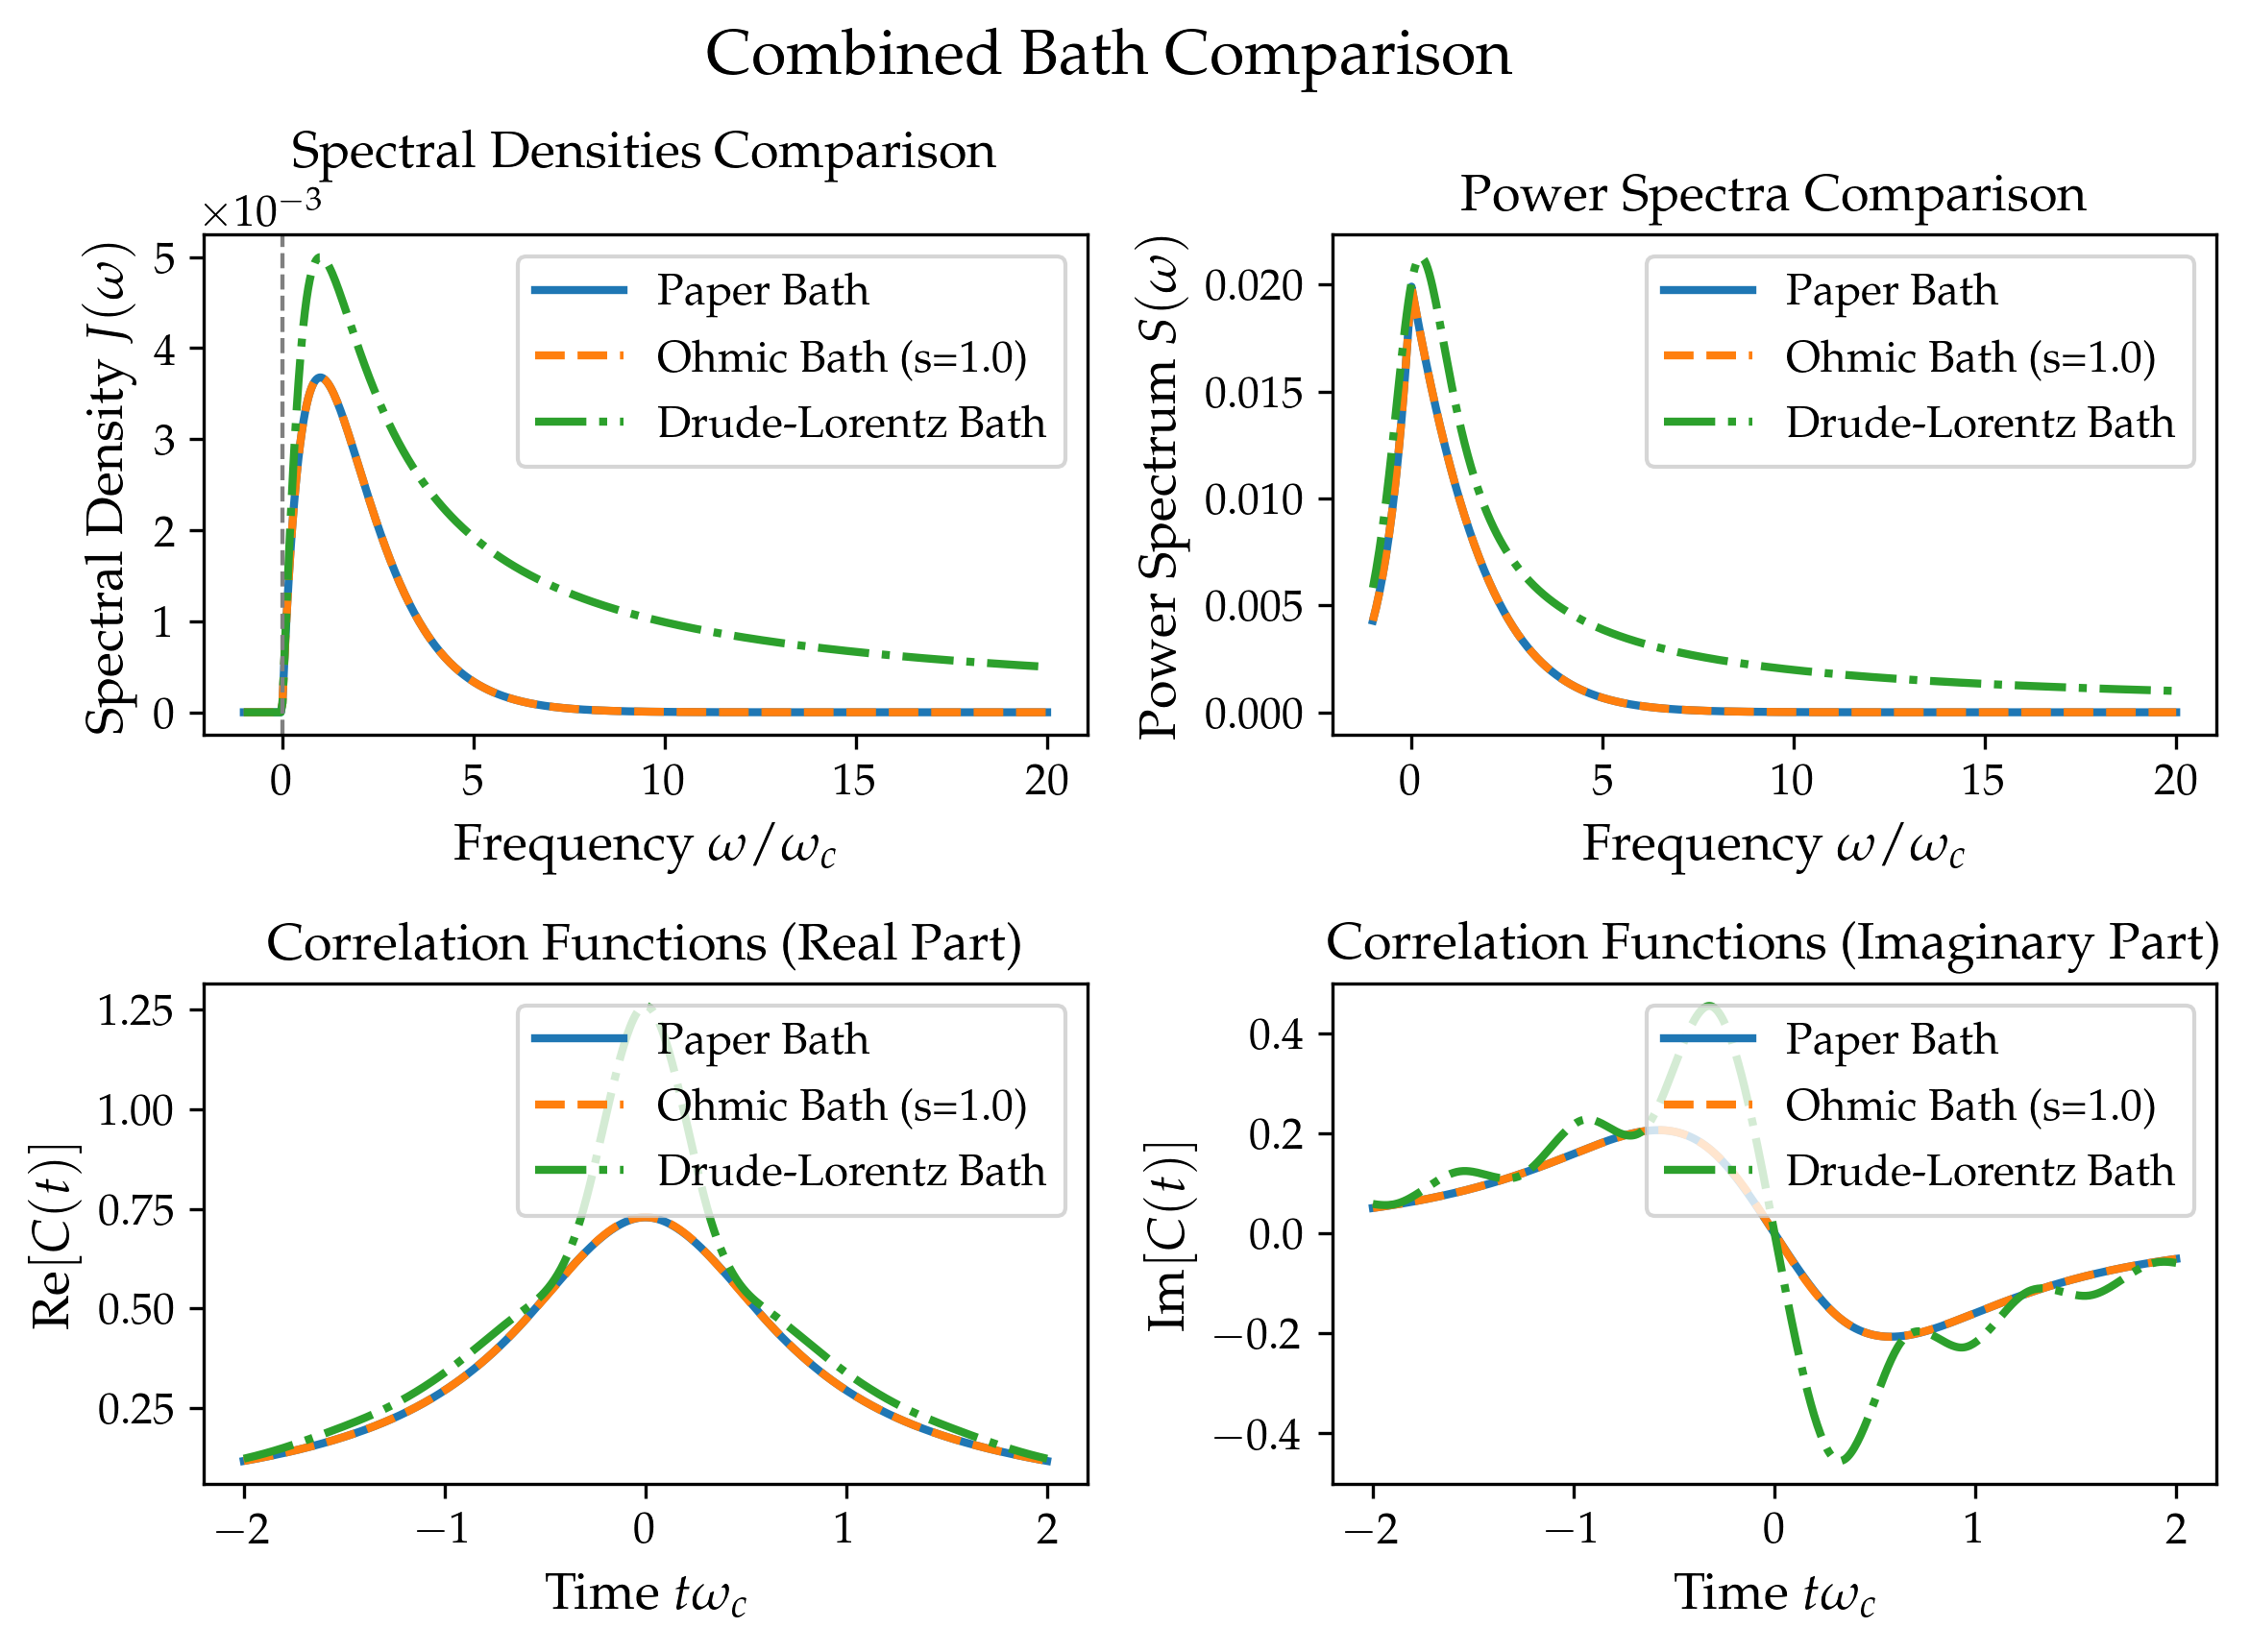
\includegraphics[width=\textwidth]{bath_comparison_combined_0.010_100.00_100.000.png}
	\caption{Comparison of representative bath models (Ohmic and Drude--Lorentz) showing spectral densities, associated power spectra, and time-domain correlation functions for coupling strength $\alpha = 0.1$, cutoff $\omega_c = 100$, and temperature $T=100$. Distinct spectral shapes map directly onto different relaxation and dephasing behaviors.}
	\label{fig:bath_comparison}
\end{figure}

% also include a temperature dep. picture
\begin{figure}
	\centering
	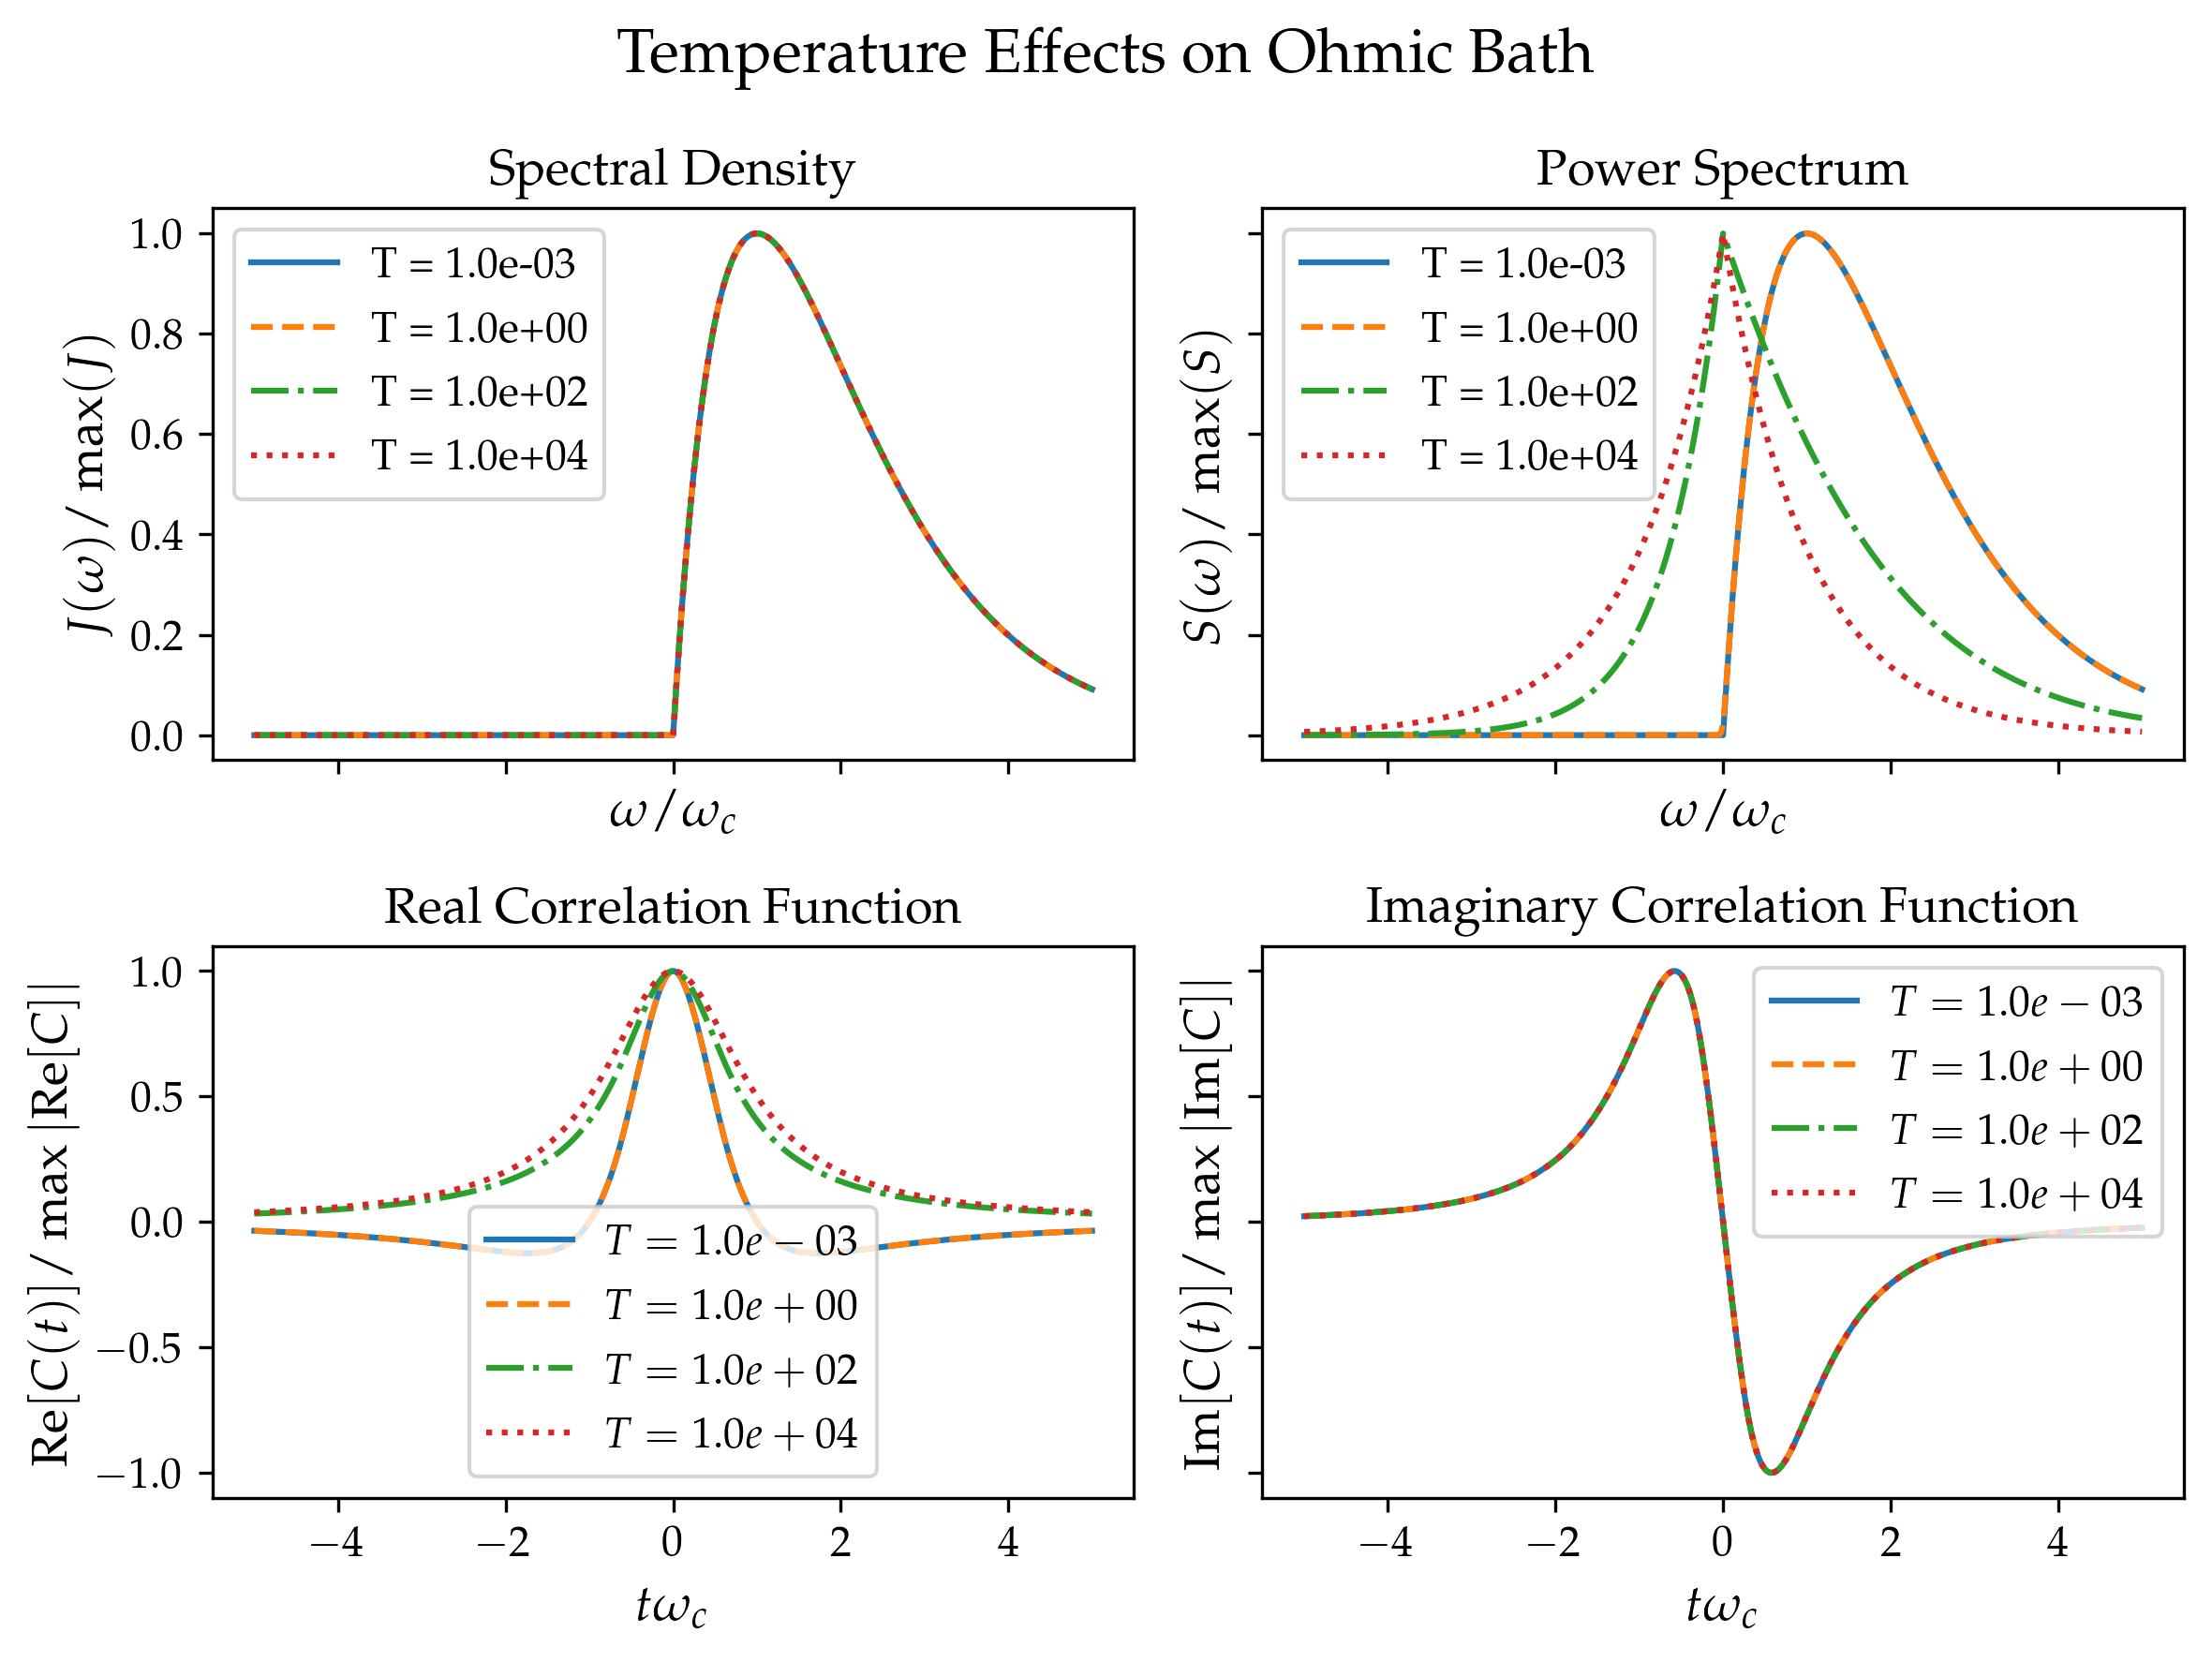
\includegraphics[width=\textwidth]{temperature_analysis_ohmic_bath.png}
	\caption{Temperature dependence of the bath correlation function for an Ohmic bath with $\alpha = 1$ and cutoff $\omega_c = 100$. Higher temperatures increase the amplitude and decrease the correlation time, reflecting enhanced thermal fluctuations.}
	\label{fig:bath_temperature_comparison}
\end{figure}